\chapter{CRYSTALLINE COHOMOLOGY, DIEUDONN\'E MODULES, AND JACOBI SUMS}\label{art-6}

\begin{center}
{\large By~ Nicholoas M. Katz}
\end{center}

\setcounter{pageoriginal}{164}
\pageoriginale

%\tableofcontents


\section*{Introduction}
\pageoriginale
Hasse \cite{art6-key20} and Hasse-Davenport \cite{art6-key21} were the first to realize the connection between exponential sums over finite fields and the theory of zeta and $L$-functions of algebraic varieties over finite fields. This connection was exploited to Weil; one of the very first applications that Weil gave of the then newly proven ``Riemann Hypothesis'' for curves over finite fields was the estimation of the absolute value of Kloosterman sums (cf \cite{art6-key46}). The basic idea (cf \cite{art6-key20}) is that by using the theory of $L$-functions, one can express the negative of such an exponential sum as the sum of certain of the reciprocal zeroes of the zeta function itself; because the magnitude of these zeroes is given by the ``Riemann Hypothesis,'' one gets an estimate. In a fixed characteristic $p$, the estimate one gets in this way for all the fintie fields $\bF_{p^{n}}$ is best possible. On the other hand, very little is known about the variation with $p$ of the absolute values, even for Kloosterman sums, though in this case there is a conjecture, of Sato-Tate type, which seems inaccessible at present.

One case in which the problem of unknown variation with $p$ does not arise is when the expression of the exponential sum as a sum of reciprocal roots of zeta reduces to a sum consisting of a {\em single} reciprocal root; then the Riemann Hypothesis tells us the exact magnitude of the exponential sum. Conversely, an elementary argument shows that in a certain sense, this is the only case in which such exact knowledge of the magnitude of exponential sums can arise, and it shows further that a theorem of Hasse-Davenport type always results from such exact knowledge. Examples of exponential sums of this sort are Gauss sums and Jacobi sums.

Honda was the first to suggest that the identification of say, Jaboci sums, with reciprocal zeroes of zeta functions could also lead to significant non-archimedean information about Jacobi sums. A few years before his untimely death, Honda conjectured a $p$-adic limit formula for Jacobi sums in terms of ratios of binomail coefficients (\cite{art6-key23}). I gave an over-complicated proof (in a letter to Honda of Nov. 1971) which managed to shed no light whatever on the meaning of the formula. Recently, B. H. Gross and N. Koblitz \cite{art6-key14} showed that Honda's limit formula was really an {\em exact} $p$-adic formula for Jacobi sums in terms of products of values of Morita's $p$-adic $\Gamma$-function; as such, it constituted the first improvement in this century over Stickelberger's formula which gave the $p$-adic\pageoriginale valuation and the {\em first} non-vanishing $p$-adic digit in the $p$-adic expansion of a Jacobi sum!

In this paper, I will discuss the cohomological genesis of formulas of the sort discovered by Honda. The basic idea is that the reciprocal zeroes of zeta are the eigenvalues of the Frobenius endomorphism of a suitable cohomology group; if this group, together with the action of Frobenius upon it, can be made sufficiently explicit, one obtains the desired ``explicit formulas''.

There are two approaches to the question, which differ more in style than in substance. The first and longer is based on Honda's explicit construction of the Dieudonn\'e module of a formal group in terms of ``formal de Rham cohomology''. The second, less elementary but more efficient, is grounded in crystalline cohomology, particularly in the theory of the de Rham-Witt complex. I hope the reader will share my belief that there is something to be gained from each of the approaches, and pardon my decision to discuss both of them.

I would like to thank B. Dwork for many helpful discussions concerning the original proof of Honda's conjecture. Whatever I know of the Grothendieck-Mazur-Messing approach to Dieudonn\'e theory through exotic Ext's, I was taught by Bill Messing. I would also like to thank Spencer Bloch for his encouragement when I was trying to understand Honda's explicit Dieudonn\'e theory, and Luc Illusie for gently correcting some extravagent assertions I made at the Colloquium.

Finally, I would like to dedicate this paper to the memory of T. Honda.

\medskip
\noindent
{\bf I. Elementary Axiomatics, and the Hasse-Davenport Theorem.}
Consider a projective, smooth and geometrically connected variety $X$, say of dimension $d$, over a finite field $\bF_{q}$. For each integer $n\geq 1$, we denote by $X(\bF_{q^{n}})$ the finite set of points of $X$ with values in $\bF_{q^{n}}$, and by $\sharp X(\bF_{q^{n}})$ the cardinality of this set. The zeta function $Z(X/\bF_{q},T)$ of $X$ over $\bF_{q}$ is the formal power series in $T$ with $Q$-coefficients defined as
$$
Z(X/\bF_{q},T)=\exp \left(\sum\limits_{n\geq 1}\frac{T^{n}}{n}\sharp X(\bF_{q^{n}})\right).
$$
Thanks\pageoriginale to Deligne \cite{art6-key6}, we know that this zeta function has a unique expression as a finite alternating product of polynomials $P_i (T) \in \bZ [T]$, $i = 0, \ldots, 2d$:
$$
Z (X/ \bF_q, T) = \prod\limits^{2d}_{i=0} P_i (T)^{(-1)^{i+1}} = \frac{P_1 P_3 \ldots P_{2d-1}}{P_0 P_2 \ldots P_{2s}}
$$
in which each polynomial $P_i (T) \in\bZ[T]$ is of the form 
$$
P_i (T) = \prod\limits^{\deg P_i}_{j=1} (1 -\alpha_{i,j} T)
$$
with $\alpha_{i,j}$ algebraic integers such that 
$$
|\alpha_{i,j}| = \sqrt{q}^i
$$
for \textit{any} archimedean absolute value $|\;|$ on the field $\bar{\bQ}$ of all algebraic numbers. The extreme polynomials $P_0$, $P_{2d}$ are given explicitly:
$$
P_0 (T) = (1-T) , P_{2d} (T) = (1 - q^d \cdot T)
$$

Despite this apparently ``elementary'' characterization of the polynomials $P_i (T)$, their true genesis is cohomological. Let us recall this briefly.

For each prime number $l$ different from the characteristic $p$ of $\bF_q$, let us denote by $H^i_l(X)$ the finitely generated $\bZ_l$-module defined as 
$$
H^i_l (X) =  \varprojlim_n H^i_{\text{etale}} (X \otimes \bar{\bF}_q, \bZ / l^n \bZ ).
$$
Corresponding to the prime $p$ itself, we denote by $W(\bF_q)$ the ring of $p$-Witt vectors of $\bF_q$, and by $H^i_{\text{cris}} (X)$ the finitely generated $W(\bF_q)$-module defined as 
$$
H^i_{\text{cris}} (X) = \varprojlim_n H^i_{\text{cris}} (X / W_n (\bF_q)).
$$
The Frobenius endomorphism $F$ of $X$ relative to $\bF_q$ acts, by functoriality, on these various cohomology groups $H^i_l(X)$ for $l\neq p$, and $H^i_{\text{cris}} (X)$; and $F$ induces automorphisms of the corresponding vector spaces $H^i_l(X) \bigotimes_{Z_l} Q_l$, $H^i_{\text{cris}} (X) \bigotimes_{W(\bF_q)} K$ ($K$ denoting the fraction field of $W(\bF_q)$). The polynomial $P_i (T) \in \bZ [T]$ which occurs in the factorization of the zeta function is then given cohomologically by the formulas 
\begin{gather*}
P_i(T) = \det (1 - T F \big| H^i_l(X) \otimes \bQ_l) \text{ for } l \neq p\\
P_i (T) = \det (1 - T F \big| H^i_{\text{cris}} (X) \otimes K).
\end{gather*}\pageoriginale 

The resulting formula for zeta as the alternating product of characteristic polynomials of $F$ on the $H^i$, in each of the cohomology theories $H^i_l (X) \otimes Q_l$ for $l \neq p$, $H^i_{\text{cris}} (X) \otimes K$, is equivalent, via logarithmic differentiation, to the identities in those theories 
$$
\neq X (\bF_{q^n}) = \sum (-1)^i \text{ trace } (F^n \big| H^i). \text{ for all } n \geq 1.
$$
By viewing the set $X(\bF_{q^n})$ as the set of fixed points of $F^n$ acting on $X(\bar{\bF}_q)$, this identity becomes a Lefschetz trace formula
$$
\# \text{ Fix } (F^n ) =\sum(-1)^i \text{ trace } (F^n \big| H^i) \text{ all } n \geq 1
$$
for $F$ and its iterates in each of our cohomology theories. If we take as \textit{given} these Lefschetz trace formulas, then the identification of $P_i$ with $\det (1 - F T \big| H^i)$ is equivalent to the assertion:
\begin{align*}
&\text{On any of the groups $H^i_l(X) \otimes Q_l$ with $l \neq p$,}\\
&\text{$H^i_{\text{cris}} (X) \otimes K$, the eigenvalues of $F$ are alge-}\\
&\text{braic integers all of whose archimedean absolute}\\
&\text{values are $\sqrt{q}^i$.}
\end{align*}
In fact, there is not a great deal more that is known about the action of $F$ on the $H^i_l(X) \otimes Q_l$ for $l \neq p$, and on $H^i_{\text{cris}} (X)  \otimes K$. It is still \textit{not} known, for example, whether the action of $F$ on these cohomology groups is always semi-simple when $i>1$. (That it is when $i =1$ results from the theory of abelian varieties).

Suppose that a finite group $G$ operates on $X$ by $\bF_q$-automorphisms. Let us choose a number field $E$ big enough that all complex representations of $G$ are realizable over $E$, and whose residue fields at all $p$-adic places contain $\bF_q$. (For example, the field $Q(\zeta_{q-1}, \zeta_N)$, where $N$ is the $l$.c.m. of the orders of elements of $G$, is such an $E$). We denote by $\lambda$ an $l$-adic place of $E$, $l \neq p$, and by $\sfP$ a $p$-adic place of $E$. Thus $E_\lambda$ is a finite extension of $Q_l$, and $E_\sfP$ is a finite extension of $K$.

Let $M$ be a finite dimensional $E$-vector space given with an action of $G$, say $\rho : G \to \Aut_E (M)$. The associated $L$-function $L(X/\sF_q, \rho, T)$ is the formal power series with $E$-coefficients defined as 
$$
L(X/\sF_q, \rho, T) = \exp \left(\sum\limits_{n \geq 1} \frac{T^n}{n} \cdot \frac{1}{\# G} \sum\limits_{g \in G} tr (\rho (g^{-1})) \# Fix (F^n g) \right)
$$\pageoriginale
where Fix $(F^n g)$ denotes the finite set of fixed points of $F^ng$ acting on $X(\bar{\bF}_q)$. We recover the zeta function of $X/\bF_q$ by taking for $\rho$ the regular representation of $G$. The usual formalism of zeta and $L$-functions gives 
$$
Z(X/ \bF_q, T) = \prod\limits_{\rho \text{ irred}} L (X / \bF_q, \rho, T)^{\deg (\rho)}
$$

It follows from Deligne's results that for any representation $\rho$, we have a unique expression for the corresponding $L$-function as an alternating product of polynomials $P_{i,\rho}(T) \in E [T]$,
$$
L(X/ \bF_{q}, \rho, T) =\prod\limits^{2d}_{i=0} P_{i,\rho} (T)^{(-1)^{i+1}},
$$
which are of the form 
$$
P_{i,\rho} (T) = \prod\limits^{\deg P_{i,\rho}}_{j=1} (1 - \alpha_{i, j, \rho} T)
$$
with algebraic integers $\alpha_{i, j,\rho}$ such that 
$$
|\alpha_{i, j, \rho}| = \sqrt{q}^i
$$
for any archimedean absolute value $|\;|$ on the field $\bar{Q}$ of all algebraic numbers. 

The cohomological expression of there $P_{i,\rho}$ is straighforward  (\cf\cite{art6-key18}). Because the action of $G$ is ``defined over $\bF_q$'' it commutes with $F$, and therefore the induced action of $G$ on the cohomology commutes with the action of $F$. Therefore $G$, acting by composition, induces automorphisms of the $E_\lambda$-vector spaces,$l \neq \rho$,
$$
\Hom_{E_\lambda [G]} (M\bigotimes\limits_E E_\lambda, H^i_l (X) \bigotimes\limits_{Z_l} E_\lambda).
$$
and of the $E_\sfP$-vector spaces
$$
\Hom_{E_{\sfP} [G]} (M \bigotimes\limits_{E} E_\sfP, H^i_{\text{cris}} (X) \bigotimes\limits_{W(\sF_q)} E_\sfP). 
$$
The polynomials $P_{i, \rho} (T) \in E [T]$ are given by the formulas 
\begin{align*}
P_{i,\rho} (T) & = \det (1 - T F \big| \Hom_{E_\lambda [G]} (M \bigotimes\limits_{E} E_\lambda, H^i_l (X) \bigotimes\limits_{Z_l} E_\lambda )) \text{ for } l \neq \rho \\
P_{i, \rho} (T) & = \det (1 - TF \big| \Hom_{E_\sfP [G]} (M\bigotimes\limits_E E_\sfP, H^i_{\text{cris}} (X) \bigotimes\limits_{W (\sF_q)} E_\sfP)).
\end{align*}

Let us\pageoriginale recall the derivation of these formulas. We first observe that the characteristic polynomial of $F$ on $\Hom_G (M, H^i) \simeq ({\displaystyle{\mathop{M}^v}} \otimes H^i)^G \subset {\displaystyle{\mathop{M}^v}} \otimes H^i$ \textit{divides} $\det (1-F T \big| H^i)^{\dim {\displaystyle{\mathop{M}^v}}}$, and hence the eigenvalues of $F$ on $\Hom_G (M, H^i)$ are algebraic integers, all of whose archimedean absolute values are $\sqrt{q}^i$. So it remains only to verify that the alternating product of those characteristic polynomials is indeed the $L$-function, \ie. that 
$$
L(X \backslash \bF_q, \rho, T) = \prod \det (1 - F T \big| ({\displaystyle{\mathop{M}^v}} \otimes H^i)^{G} )^{(-1)^{i+1} },
$$
Equivalently, we must check that 
\begin{align*}
\frac{1}{\# G} \sum \text{ trace }\rho  (g^{-1}) &\;\# \text{ Fix } (F^n g)\\
& = \sum (-1)^i \text{ trace } (1 \otimes F^n \big| ({\displaystyle{\mathop{M}^v}} \otimes H^i)^G)\\
& = \sum (-1)^i \frac{1}{\# G} \sum\limits_{g \in G} \text{ trace } (g \otimes F^n g \big|{\displaystyle{\mathop{M}^v}} \otimes H^i)\\
& = \sum (-1)^{i} \frac{1}{\# G} \sum\limits_{g \in G} \text{ trace } {\displaystyle{\mathop{\rho}^v}} (g) \cdot \text{ trace } (F^n g \big| H^i)\\
& = \frac{1}{\# G} \sum\limits_{g \in G}  \text{ trace } \rho (g^{-1}) \sum (-1)^i \text{ trace } (F^n g \big| H^i). 
\end{align*}
To check this last equality, we would like to invoke the Lefschetz trace formula, not for $F^n$, but for $F^ng$, with $g$ an automorphism of \textit{finite order} which commutes with $F$; this amounts to invoking the Lefschetz trace formula for $Fg$ on $X$ and on all its ``extensions of scalars'' $X \otimes \bF_{q^n}$. But an elementary descent argument shows that given an automorphism $g$ of finite order which commutes with $F$, there is \textit{another} variety $X'/ \bF_q$ together with an isomorphism $X \otimes \bar{\bF}_q \simeq X' \otimes \bar{\bF}_q$ under which $F g \otimes 1$ corresponds to $F \otimes 1$. Because this isomorphism also induces isomorphisms of cohomology groups 
\begin{gather*}
H^i_l (X)^{\text{dfn}} H^i_{\text{et}} (X' \otimes \bar{\bF}_q, \bZ_l) \simeq H^i (X \otimes \bar{\bF}_q, \bZ_l)^{\text{dfn}} H^i_l(X),\\
H^i_{\text{cris}} (X') \otimes W (\bar{\bF}_q) \simeq H^i_{\text{cris}} (X' \otimes \bar{\bF}_q) \simeq H^i_{\text{cris}} (X \otimes \bar{\bF}_q) \simeq\\
\simeq H^i_{\text{cris}} (X) \otimes W (\bar{\bF}_q),
\end{gather*}
the truth\pageoriginale of the Lefschetz formula for $Fg$ on $X$ results from its truth for $F$ on $X'$.

Let us now consider in greater detail the case of an irreducible $\rho$. Then $P_{i, \rho}$ is a polynomial whose degree is the common \textit{multiplicity} of $\rho$ in any of the $H^i_l(X) \otimes E_\lambda$, $l \neq \rho$, or in $H^i_{\text{cris}} (X) \otimes E_\sfP$. Decomposing the regular representation leads to the factorization
$$
P_i (T) = \prod\limits_{\rho \text{ irred}} P_{i, \rho} (T)^{\deg (\rho)}
$$
The coarser factorization 
$$
P_i (T) = \prod\limits_{ \rho \text{irred}} (P_{i,\rho} (T)^{\deg(\rho)})
$$
corresponds to the decomposition of $H^i_l(X) \otimes E_\lambda$, $\resp H^i_{\text{cris}} (X) \otimes E_\sfP$, into $\rho$-isotypical components
\begin{gather*}
H^i_l (X) \otimes E_\lambda \simeq \bigotimes\limits_{\text{irred} \rho } \left(H^i_l(X) \times E_\lambda \right)^\rho\\
H^i_{\text{cris}} (X) \otimes E_\sfP \simeq \bigotimes\limits_{\text{irred} \rho} \left(H^i_{\text{cris}} (X) \otimes E_\sfP \right)^\rho
\end{gather*}
Indeed the corresponding identities, for $\rho$ irreducible, are 
\begin{align*}
P_{i,\rho} (T)^{\deg(\rho)}  & = \det (1 - TF \big| (H^i_l (X) \otimes E_\lambda)^\rho) l \neq p\\
P_{i, \rho} (T)^{\deg (\rho)} & = \det (1 - TF \big| (H^i_{\text{cris}} (X) \otimes E_\sfP)^\rho).
\end{align*}

Let us denote by $S(X/ \bF_q, \rho, n)$ the exponential sums used to define the $L$-function:
$$
S (X/ \sF_q , \rho, n) = \frac{1}{\# G} \sum\limits_{g \in G} tr (\rho (g)) \# \text{ Fix }(F^n g^{-1}). 
$$
The following lemma gives the cohomological meaning of theorems of Hasse-Davenport type (\cf \cite{art6-key20}).

\medskip
\noindent
{\bfseries Lemma \thnum{1.1}:\label{art6-lem1.1}}
\textit{Let $X/\bF_q$ be projective and smooth. Let a finite group $G$ operate on $X$ by $\bF_q$-automorphisms, and let $p$ be an irreducible complex representation of $G$. Fix an integer $i_\circ$, and denote by $H^{i_\circ}$ any one of the cohomology groups $H^{i_\circ}_l(X) \bigotimes_{Z_l} E_\lambda$ with $l \neq p$, or $H^{i_\circ}_{\text{cris}}(X) \bigotimes\limits_{W(\bF_q)} E_\sfP$. Let $|\;|$ be any archimedean absolute value on the filed $\bar{Q}$ of all algebraic numbers. The following conditions are equivalent:}
\begin{enumerate}
\item[(1)] \textit{The\pageoriginale multiplicity of $\rho$ in $H^{i_\circ}$ is one, and the multiplicity of $\rho$ in $H^i$ is zero if $i \neq i_\circ$.}

\item[(2)] \textit{For all $n \geq 1$, we have }
\begin{gather*}
(-1)^{i_\circ} S (X / \bF_q, \rho,n) = ((-1)^{i_\circ} S (X / \bF_q, \rho, 1))^n,\\
\text{and } \hspace{3cm}|S (X / \bF_q, \rho, 1)| = \sqrt{q}^{i_\circ} \hspace{3cm}
\end{gather*}

\item[(3)] \textit{For all $n \geq 1$, we have}
$$
|S(X/ \bF_q, \rho, n)| = \sqrt{q}^{i_\circ n}
$$

\item[(4)] \textit{For all $n \geq 1$, we have }
\begin{gather*}
|S (X/ \bF_q, \rho, n)| = |S(X/ \bF_q,  \rho, 1)|^n\\
\text{and } \hspace{3cm} \sqrt{q}^{i_\circ} \leq |S (X / \bF_q, \rho, 1)| < \sqrt{q}^{1+ i_\circ}\hspace{3cm}
\end{gather*}

\item[(5)] \textit{The polynomial $P_{i_{\circ, \rho}} (T)$ is given by}
$$
P_{i_{\circ, \rho}} (T) = 1 - (-1)^{i_\circ} S (X / \bF_q, \rho, 1) T 
$$
\textit{and for $i \neq i_\circ$, we have $P_{i,\rho} (T) =1$.}

\item[(6)] \textit{The $\rho$-isotypical component $(H^i)^\rho =0$ for $i \neq i_\circ$, $(H^{i_\circ})^\rho$ has dimension $ = \deg (\rho)$, and $F$ operates on $(H^{i_\circ})^\rho$ as the scalar $(-1)^{i_\circ} S (X/ \bF_q, \rho, 1)$.}
\end{enumerate}

\begin{proof}
This is an easy exercise, using the basic identities:
$$
\left\{
\begin{aligned}
&\exp \left(\sum \frac{T^n}{n}  S (X / \bF_q, \rho, n)\right) = L (X/ \bF_q, \rho, T) = \prod\limits_{i} P_{i,\rho} (T)^{(-1)^{i+1}}\\
& \quad P_{i,\rho} (T) = \prod\limits_j (1 - \alpha_{i,j,\rho} T), |\alpha_{i,j,\rho}| = \sqrt{q}^i\\
& \deg P_{i,\rho} = \textit{ multiplicity of $\rho$ in } H^i = \frac{1}{\deg (\rho)} \cdot \dim ((H^i)\rho).
\end{aligned}
\right.
$$

Suppose, first, that (1) holds, or equivalently that for $i \neq i_\circ$, $P_{i,\rho} (T) =1$, while $P_{i_{\circ, \rho}}$ is a linear polynomial $P_{i_{\circ,\rho}} (T) = (1-A T)$ with $|A| = \sqrt{q}^{i_\circ}$. The cohomological expression for $L$ then becomes 
$$
\exp \left(\sum \frac{T^n}{n} S (X/ \bF_q, \rho, n) \right) = \left(\frac{1}{1-AT} \right)^{(-1)^{i_\circ}}.
$$
Taking\pageoriginale logarithms and equating coefficients, we find 
$$
(-1)^{i_\circ} S (X/ \bF_q, \rho, n) = A^n \quad \text{ for all } n \geq 1. 
$$
 
In particular (2) and (5) hold.

The implications (5) $\Rightarrow$ (1), (6) $\Rightarrow$ (1) are obvious. Also (5) $\Rightarrow$ (6), for if $P_{i_{\circ, \rho}}$ is linear, then $\rho$ has multiplicity one in $H^{i_\circ}$, so that $(H^{i_\circ})^\rho$ is $G$-irreducible, and hence $F$ must operate on $(H^{i_\circ})^\rho$ as a \textit{scalar}, which we compute by the formula
$$
P_{i_{\circ, \rho}} (T)^{\deg (\rho)} = \det (1 - TF \big| (H^{i_\circ})^\rho).
$$

Clearly we have (2) $\Rightarrow$ (3) $\Rightarrow$ (4). We must show that if (4) holds, then exactly \textit{one} of the $P_{i,\rho}$ is $\neq 1$, and that one is linear. Logarithmically differentiating the cohomological formula for $L$, we find 
$$
S(X/ \bF_q, \rho, n) = \sum\limits_i (-1)^i \sum\limits^{\deg P_{i, \rho}}_{j=1} (\alpha_{i, j, \rho})^n, \quad |\alpha_{i,j,\rho}| = \sqrt{q}^i.
$$
We must show that if (4) holds, then the double sum has only a single term in it. Separating the $\alpha_{i, j, \rho}$ according to the \textit{parity} of $i$, we get two disjoint sets of non-zero complex numbers (disjoint because their absolute values are disjoint), to which we apply the following lemma.
\end{proof}

\medskip
\noindent
{\bfseries Lemma \thnum{1.2}:\label{art11-lem1.2}}~{\em Let $N\geq 0$ and $M\geq 0$ be non-negative integers. Let $\{A_{i}\}$ be a family of $N$ not-necessarily distinct elements of $C^{x}$, and $\{B_{i}\}$ a family of $M$ not-necessarily distinct elements of $C^{x}$. Suppose that for all $i$, $j$, $A_{i}\neq B_{j}$. If, for some real number $R>0$, we have}
$$
\left| \sum A^{n}_{j}-\sum B^{n}_{j}\right|=R^{n}\quad \text{\em for all $n\geq 1$,}
$$
{\em then $N+M=1$, i.e. either there is just one $A$ and no $B$'s, or just one $B$ and no $A$'s.}
\smallskip

\begin{proof}
Suppose first that either $N=0$ or $M=0$, say $M=0$. Then we have
$$
\left| \sum A^{n}_{i}\right|=R^{n}.
$$
Squaring, we get
$$
\sum\limits_{ij}(A_{i}\overline{A}_{j})^{n}=(R^{2})^{n}\quad\text{for}\quad n\geq 1
$$
whence\pageoriginale
$$
\prod\limits_{ij}(1-A_{i}\overline{A}_{j}T)=(1-R^{2}T),
$$
and hence $N=1$.

In case both $N\geq 1$ and $M\geq 1$, squaring leads to
$$
\sum (A_{i}\overline{A}_{k})^{n}+\sum(B_{j}\overline{B}_{l})^{n}=(R^{2})^{n}+\sum(A_{i}\overline{B}_{j})^{n}+\sum (\overline{A}_{i}B_{j})^{n}
$$
or equivalently,
$$
\frac{1}{(1-R^{2}T)}=\frac{\prod (1-A_{i}\overline{B}_{j}T)\prod(1-\overline{A}_{i}B_{j}T)}{\prod(1-A_{i}\overline{A}_{k}T)\prod(1-B_{j}\overline{B}_{l}T)}
$$
Let $R_{\max}$ be $\max (|A_{i}|,|B_{j}|)$, and consider the order of pole at $T=R^{-2}_{\max}$. The numerator's factors $1-A_{i}\overline{B}_{j}T$, $1-\overline{A}_{i}B_{j}T$ are all non-zero there (for if $A_{i}\overline{B}_{j}=R^{2}_{\max}$, by maximality we must have $A_{i}=B_{j}=R_{\max}$, in which case we see, using polar coordinates, that $A_{i}-B_{j}$, which is forbidden). In the denominator, each of the terms $(1-|A_{i}|^{2}T)$, $(1-|B_{j}|^{2}T)$ with $|A_{i}|=R_{\max}$ and $|B_{j}|=R_{\max}$ vanishes at $T=R^{-2}_{\max}$. Therefore we may conclude that in fact $R=R_{\max}$, and that precisely {\em one} among all the $A_{i}$ and $B_{j}$ has this absolute value. A similar argument shows that $R_{\min}=R$.
\end{proof}

In a similar but lighter vein, we have the following variant, whose proof is left to the reader.

\medskip
\noindent
{\bf Lemma \thnum{1.3}.\label{art6-lem1.3}}~{\em Let $X/F_{q}$ be projective and smooth. Let a finite group $G$ operate on $X$ by $F_{q}$-automorphisms, and let $\rho$ be an irreducible complex representation of $G$. Denote by $H^{i}$ any of the cohomology groups $\foprod{H^{i}_{l}(X)}{E_{\lambda}}{Z_{l}}$ with $l\neq p$, or $\foprod{H^{i}_{\text{cirs}}(X)}{E_{P}}{W}$. The following conditions are equivalent.}
\begin{itemize}
\item[(1)] {\em For all $i$, $\rho$ does not occur in $H^{i}$, i.e. we have $(H^{i})^{\rho}=0$.}

\item[(2)] {\em For all $n\geq 1$, we have}
$$
S(X/F_{q},\rho,n)=0.
$$
\end{itemize}

\bigskip
\noindent
{\bf II. Gauss\pageoriginale and Jacobi Sums as exponential sums, and as eigenvalues of Frobenius}
\smallskip

We begin by discussing Gauss sums. Let us fix an integer $N\geq 2$ prime to $p$, and a number field $E$ containing the Np'th roots of unity. Given an additive character $\psi$ of $F_{p}$, i.e. a homomorphism
$$
\psi : (F_{p},+)\to E^{\times},
$$
we define an additive character $\psi_{q}$ of each finite extension $F_{q}$ by composing $\psi$ with the trace map:
\begin{figure}[H]
\centering
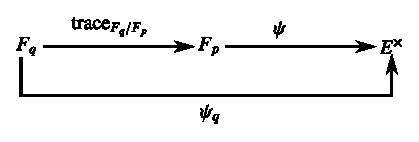
\includegraphics{chap6/fig1.eps}
\end{figure}
Given a character of $\mu_{N}$, i.e. a homomorphism
$$
\chi : \mu_{N}(E)\to E^{\times},
$$
a $p$-adic place $\sfP$ of $E$, with residue field $F_{N(P)}$, and a finite extension $F_{q}$ of this residue field, the map ``reduction mod $\sfP$'' induces an isomorphism
$$
\mu_{N}(E)\xrightarrow{\sim}\mu_{N}(F_{N(P)})=\mu_{N}(F_{q})
$$
Because $F^{\times}_{q}$ is cyclic, we know that $q\equiv 1\mod N$, and that the map $x\to x^{\frac{q-1}{N}}$ defines a surjection
$$
F^{\times}_{q}\twoheadrightarrow \mu_{N}(F_{q})=\mu_{N}(F_{N(P)})\xrightarrow{\sim}\mu_{N}(E)
$$
We define the character $\chi_{q}$ of $F^{\times}_{q}$ as the composite
\begin{figure}[H]
\centering
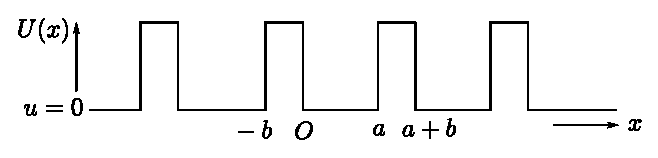
\includegraphics{chap6/fig2.eps}
\end{figure}
The Gauss sum $g_{q}(\psi,\chi,\sfP)$ attached to this situation is defined by the formual
$$
g_{q}(\psi,\chi,\sfP)=\sum\limits_{x\in F^{\times}_{q}}\psi_{q}(x)\chi_{q}(x)
$$
An\pageoriginale elementary computation shows that
$$
g_{q}(\psi,\chi,\sfP)=
\begin{cases}
q-1 & \text{if $\psi$, $\chi$ both trivial}\\
0   & \text{if $\psi$ trivial, $\chi$ non-trivial}\\
-1  & \text{if $\psi$ non-trivial, $\chi$ trivial}
\end{cases}
$$
while
$$
|g_{q}(\psi,\chi,\sfP)|=\sqrt{q}\text{~~ if~~ } \psi,\chi\text{~ both non-trivial}
$$
for any archimedean absolute value on $E$ (cf \cite{art6-key47}).

Now consider the Artin-Schreier curve $X/F_{q}$, defined to be the complete non-singular model of the affine smooth geometrically connected curve over $F_{q}$ with equation
$$
T^{P}-T=X^{N}.
$$
Set theoretically, $X$ consists of this affine curve plus a single rational point at $\infty$. The group $F_{q}\times \mu_{N}(F_{q})$ operates on $X/F_{q}$ curve by the affine formulas
$$
(a,\zeta):(T,X)\to (T+a,\zeta X),
$$
fixing the point at $\infty$. Via the ``reduction mod $\sfP$'' isomorphism
$$
\mu_{N}(E)\xrightarrow{\sim}\mu_{N}(F_{N(\sfP)})=\mu_{N}(F_{q}),
$$
we may view $(\psi,\chi)$ as a character of the group $F_{p}\times \mu_{N}(F_{q})$:
$$
(\psi,\chi)(a,\zeta)=\psi(a)\chi(\zeta).
$$
Thus we may speak of the sums
$$
S(X/F_{q},(\psi,\chi),n)=\frac{1}{pN}\sum\limits_{(a,\zeta)\in F_{p}\times \mu_{N}}\psi(a)\chi(\zeta)\sharp \text{~Fix~} (F^{n}\cdot (a,\zeta)^{-1})
$$
attached to this situation.

\medskip
\noindent
{\bf Lemma \thnum{2.1}.\label{art6-lem2.1}}~{\em If $\chi$ is non-trivial and $\psi$ is arbitrary, then we have}
\begin{equation*}
S(X/F_{q},(\psi,\chi),n)=g_{q^{n}}(\psi,\chi,\sfP).\tag{2.1.1}\label{art6-eq2.1.1}
\end{equation*}

\begin{proof}
It\pageoriginale suffices to treat the case $n=1$, for we have
$$
S(X/F_{q^{n}},(\psi,\chi),1)=S(X/F_{q},(\psi,\chi),n).
$$
We can rewrite $S(X/F_{q},(\psi,\chi),1)$ as
$$
\sum\limits_{x\in X(\overline{F}q)}\frac{1}{pN}\sum\limits_{\substack{(a,\zeta)s.t.\\ F(x)=(a,\zeta)(x)}}\psi(a)\chi(\zeta)
$$
Given any point $x\in X(\overline{F}_{q})$, the set of $(a,\zeta)\in F_{p}\times \mu_{N}$ which satisfy $F(x)=(a,\zeta)(x)$ is either empty or principal homogeneous under the inertia {\em subgroup} $I_{x}$ of $F_{p}\times \mu_{N}$ which {\em fixes} $x$; therefore if the restriction of $(\psi,\chi)$ to this subgroup is {\em non-trivial}, the inner sum above {\em vanishes}. Because $\chi$ is assumed {\em non-trivial}, this vanishing applies to the point at $\infty$ (for which $I_{x}$ is all of $F_{p}\times \mu_{N}$) and to any finite point $(T,0)$ whose $X$-coordinate is zero (then $I_{(T,0)}=\{0\}\times \mu_{N}$).

Given a point $(T,X)$ with $X\neq 0$, we have
$$
F(T,X)=(T^{q},X^{q})
$$
and the inertia subgroup $I_{(T,X)}$ is trival. If there is an element $(a,\zeta)\in F_{p}\times \mu_{N}$ satisfying $F(T,X)=(T+a,\zeta X)$, then it is given by the formulas
$$
a=T^{q}-T, \ \zeta=X^{q-1}
$$
Since the point $(T,X)$ is subject to the defining equation
$$
T^{p}-T=X^{N}
$$
we see that
\begin{align*}
& (X^{N})^{q-1}=(X^{q-1})^{N}=\zeta^{N}=1,\text{~ hence~ } X^{N}\in F^{\times}_{q}, \ \zeta=(X^{N})^{\frac{q-1}{N}}\\[3pt]
& T^{p}-T=X^{N}\in F^{\times}_{q},\\[3pt]
& a=T^{q}-T=\text{~trace}_{F_{q}/F_{p}}(T^{p}-T)=\text{trace}_{F_{q}/F_{p}}(X^{N}).
\end{align*}
For each $u\in F^{\times}_{q}$, the equations $(T^{P}-T=u,X^{N}=u)$ have $pN$ solutions $(T,X)$ over $\overline{F}_{q}$, all of which satisfy
$$
F(T,X)=(a,\zeta)(T,X)
$$
with\pageoriginale the {\em same} $(a,\zeta)$, namely (trace$_{F_{q}/F_{p}}(u)$, $u^{\frac{q-1}{N}}$), and {\em every} point $(T,X)$ which contributes to our sum lies over some $u\in F^{\times}_{q}$. Thus our sum becomes
$$
\sum\limits_{u\in F^{\times}_{q}}\psi(\text{trace}_{F_{q}/F_{p}}(u))\chi(u^{\frac{q-1}{N}})^{\text{dfn}}g_{q}(\psi,\chi,\sfP).
$$
\end{proof}

\medskip
\noindent
{\bf Corollary \thnum{2.2}.\label{art6-coro2.2}}~{\em Let $H^{i}$ denote any of the cohomology groups $H^{i}_{l}(X)\otimes E_{\lambda}$ with $l\neq p$, or $\foprod{H^{i}_{\text{cris}}(X)}{E_{P}}{W}$ of the Artin Schreier curve $X/F_{q}$.}
\begin{itemize}
\item[(1)] {\em If $\psi$ and $\chi$ are both non-trivial, then the eigenspace $(H^{1})^{\psi\cdot \chi}$ is one-dimensional, and we have a direct sum decomposition}
$$
H^{i}=\oplus (H^{1})^{\psi\cdot \chi}
$$
{\em indexed by the ($p-1(N-1)$ pairs $(\psi,\chi)$) of non-trivial characters.}

\item[(2)] {\em The eigenvalue of $F$ on $(H^{1})^{\psi\cdot \chi}$ is $-g_{q}(\psi,\chi,\sfP)$, and for each $n\geq 1$ we have the Hasse-Davenport formula}
$$
-g_{q^{n}}(\psi,\chi,\sfP)=(-g_{q}(\psi,\chi,\sfP))^{n}.
$$

\item[(3)] {\em The group $F_{q}\times \mu_{N}$ acts trivially on both $H^{0}$ and $H^{2}$.}
\end{itemize}

\begin{proof}
That the group acts trivially on both $H^{0}$ and $H^{2}$ follows from the fact that these are one-dimensional spaces on which $F$ always acts as $1$ and $q$ respectively. The descent argument shows that for any automorphism of {\em finite order} $g$ which commutes with $F$, $Fg$ also acts as $1$ and $q$ on $H^{0}$ and $H^{2}$ respectively, and hence that $g$ itself acts trivially on $H^{0}$ and $H^{2}$.

That the multiplicity of $(\psi,\chi)$ in $H^{1}$ is {\em one} when both $\psi$ and $\chi$ are non-trivial follows from the lemma of the previous section, given the identity \eqref{art6-eq2.1.1} and the known absolute value of gauss sums; and assertion (2) above is just a repetition of part of that lemma in this particular case. To see that no other characters occurs in $H^{1}$, we recall that the dimension of $H^{1}$ is known to be $2g$, $g=$ genus of $X$, and so it suffices to verify that $2g=(p-1)(N-1)$. This formula, whose elementary verification we leave to the reader, is in fact valid in any characteristic prime to $N(p-1)$. (Hing: view $T^{P}-T=X^{N}$ an an $N$-fold covering of the $T$-line!)
\end{proof}

We\pageoriginale now turn to the consideration of Jacobi sums. We fix an integer $N\geq 2$ prime to $p$, and a number field $E$ containing the $N$'th roots of unity. Given a $p$-adic place $\sfP$ of $E$, a character $\chi$ of $\mu_{N}$
$$
\chi :\mu_{N}(E)\to E^{\times}
$$
and a finite extension $F_{q}$ of the residue field $F_{N(\sfP)}$ at $\sfP$, we obtain the character $\chi_{q}$
$$
\chi_{q}:F^{\times}_{q}\to E^{\times}
$$
in the manner explained above. Given two characters $\chi$, $\chi'$ of $\mu_{N}$, the Jacobi sum $J_{q}(\chi,\chi',\sfP)$ is defined by the formula
$$
J_{q}(\chi,\chi',\sfP) {\displaystyle{\mathop{=}\limits^{\text{dfn}}}}\sum\limits_{\substack{x\in Fq\\ x\neq 0,1}}\chi_{q}(x)\chi'_{q}(1-x).
$$
An elementary computation (cf \cite{art6-key14}) shows that if the {\em product} $\chi\chi'$ is non-trivial, then for any non-trivial additive character $\psi$ of $F_{p}$, we have the formula
$$
g_{q}(\psi,\chi,\sfP)g_{q}(\psi,\chi',\sfP)=J_{q}(\chi,\chi',\sfP)g_{q}(\psi,\chi\chi',\sfP)
$$
In particular, from the known absolute values of Gauss sums we obtain
$$
|J_{q}(\chi,\chi',\sfp)|=\sqrt{q}
$$
for all archimedean absolute values of $E$, provided that $\chi$, $\chi'$, and $\chi\chi'$ are {\em all} non-trivial.

Now consider the Fermat curve $Y/F_{q}$, defined by the homogeneous equation
$$
X^{N}+Y^{N}=Z^{N}
$$
The group $\mu_{N}\times \mu_{N}$ operates on this curve by the formula
$$
(\zeta_{1},\zeta_{2}):(X,Y,Z)\to (\zeta_{1}X,\zeta_{2}Y,Z).
$$
Viewing $(\chi,\chi')$ as a character of this group
$$
(\chi,\chi')(\zeta_{1},\zeta_{2}) {\displaystyle{\mathop{=}\limits^{\text{dfn}}}}\chi(\zeta_{1})\chi'(\zeta_{2}),
$$
we may speak of the sums $S(Y/F_{q},(\chi,\chi')n)$ attached to this situation.

In\pageoriginale complete analogy with the situation for the Artin-Schreier curve, we have the following lemma and corollary, whose analogous proofs are left to the reader.

\medskip
\noindent
{\bf Lemma \thnum{2.3}.\label{art6-lem2.3}}~{\em If $\chi$ and $\chi'$ are non-trivial characters of $\mu_{N}$ such that $\chi\chi'$ is also non-trivial, then we have, for all $n\geq 1$,}
\begin{equation*}
S(Y/F_{q},(\chi,\chi'),n)=J_{q^{n}}(\chi,\chi',\sfp).\tag{2.3.1}\label{art6-eq2.3.1}
\end{equation*}
\smallskip

\noindent
{\bf Corollary \thnum{2.4}.\label{art6-coro2.4}}~{\em Let $H^{i}$ denote any of the cohomology groups $H^{i}_{l}(Y)\otimes E_{\lambda}$ with $l\neq p$, or $\foprod{H^{i}_{\text{cris}}(X)}{E_{\sfp}}{W}$ of the Fermat curve $Y/F_{q}$.}
\begin{itemize}
\item[(1)] {\em If $\chi$, $\chi'$ and $\chi\chi'$ are all non-trivial, then the eigenspace $(H^{1})^{(\chi,\chi')}$ is one-dimensional, and we have a direct sum decomposition}
$$
H^{1}=\oplus (H^{1})^{(\chi,\chi')}
$$
{\em indexed by the $(N-1)(N-2)$ pairs $(\chi,\chi')$ of non-trivial characters of $\mu_{N}$ whose product $\chi\chi'$ is also non-trivial}.

\item[(2)] {\em The eigenvalue of $F$ on $(H^{1})^{(\chi,\chi')}$ is $-J_{q}(\chi,\chi',\sfP)$, and for each integer $n\geq 1$ we have the Hasse-Davenport formula}
$$
-J_{q^{n}}(\chi,\chi',\sfP)=(-J_{q}(\chi,\chi',\sfP))^{n}.
$$

\item[(3)] {\em The group $\mu_{N}\times \mu_{N}$ operates trivially on both $H^{0}$ and $H^{2}$.}
\end{itemize}

\bigskip
\noindent
{\bf III. The problem of ``explicitly'' computing Frobenius.} We return now to the general setting of a projective, smooth, and geometrically connected variety $X/F_{q}$ of dimension $d$. A tantalizing feature of all the cohomology theories that we have been discussing is that when the variety $X$ ``lifts'' to characteristic zero, then the corresponding cohomology groups $H^{i}(X)$ have an ``elementary'' description in terms of standard algebro-geometric and topological invariants of the lifting.

More precisely, suppose we are given a projective smooth scheme $X$ over $W(F_{q})$, together with an $F_{q}$-isomorphism of its special fibre with $X$. (This is a rather strong notion of what a ``lifting'' of $X$ should mean, but it is adequate for our purposes, and it avoids certain technical problems related to ramification). Then there is a canonical isomorphism
$$
H^{i}_{\text{cris}}\to H^{i}_{\DR}(X/W(F_{q}))
$$
of\pageoriginale $H^{i}_{\text{cris}}$ with the algebraic de Rham cohomology of the lifting (cf \cite{art6-key19}, \cite{art6-key27}).

To discuss $H^{i}_{l}(X)$, we must in addition choose (!) a complex embedding
$$
W(F_{q})\hookrightarrow C.
$$
By means of such an embedding, we may ``extend scalars'' to obtain from $X/W$ a projective smooth complex variety $X_{C}$, and an associated complex manifold $X^{\text{an}}_{C}$. For each prime number $l\neq p$, there is a canonical isomorphism
$$
H^{i}_{l}(X)\to \fprod{H^{i}_{\text{top}}(X^{\text{an}}_{C},Z)}{Z_{l}}{Z},
$$
where $H^{i}_{\text{top}}$ denotes the usual ``topological'' cohomology.

To emphasize the similarity between these two sorts of isomorphisms, recall that by GAGA and the holomorphic Poincar\'e lemma, we have a canonical isomorphism
\[
\xymatrix{
\foprod{H^{i}_{\DR}(X/W)}{C}{W}\ar[r]^{\sim} & H^{i}_{\DR}(X/C)\ar[r]^{\sim} & H^{i}_{\top}(X^{an}_{C},C)\\
                                         &                           & \foprod{H^{i}_{\top}(X^{an},Z)}{C}{Z}\ar[u]^{\rotatebox{90}{$\backsim$}}
}
\]

Unfortunately, these rather concrete descriptions of the various cohomology {\em groups} $H^{i}(X)$ shed little light on their {\em functoriality}. In the rather unusual case of an $F_{q}$-endomorphism $f:X\to X$ which happens to admit a lifting to a $W$-endomorphism
$$
f:X\to X,
$$
we have the simple formulas
$$
\begin{cases}
f^{*}\text{~ on~ } H^{i}_{\text{cris}}(X)=f^{*}\text{~ on~ } H^{i}_{\DR}(X/W)\\
f^{*}\text{~ on~ } H^{i}_{l}(X)=(f^{an}_{C})^{*}\otimes 1\text{~ on~ } \foprod{H^{i}_{\top}(X^{an}_{C},Z)}{Z_{l},l\neq p}{Z}
\end{cases}
$$
But for those $f$ which do not lift, we are left somewhat in the dark as to an explicit description of the map $f^{*}$ on cohomology.

Suppose for example that a finite group $G$ operates on $X$ by $F_{q}$-automorphisms, and that this action can be lifted to an action of $G$ on $X$ by $W$-automorphisms. Then our canonical isomorphisms
$$
\begin{cases}
H^{i}_{\text{cris}}(X)\xrightarrow{\sim} H^{i}_{\DR}(X/W)\\
H^{i}_{l}(X)\xrightarrow{\sim} H^{i}_{\top}(X^{an}_{C},Z)\otimes Z_{l}\text{~ for~ } l\neq p
\end{cases}
$$\pageoriginale
are $G$-equivariant. In particular, we can ``explicitly compute'' the multiplicities of the various complex irreducible representations $\rho$ of $G$ in the cohomology of $X$, and we can ``explicitly compute'' the various isotypical components of the cohomology. If it turns out that a given irreducible representation $\rho$ occurs in a given $H^{i}$ with multiplicity {\em one}, then we know a priori that $F$ must operate on the corresponding isotypical component $(H^{i})^{\rho}$ as a {\em scalar}, and we know this even when $F$ itself does not lift.

For example, we could recover the isotypical decomposition of $H^{1}$ of the Fermat curve $Y$ under the action of $\mu_{N}\times \mu_{N}$ by lifting the curve and the group action (use the ``same'' equations) and making an explicit algebro-geometric or topological calculation of the corresponding isotypical decomposition in characteristic zero. In terms of, say, the crystalline cohomology, we obtain an $F$-stable decomposition
$$
H^{1}_{\text{cris}}(Y)\xrightarrow{\sim}H^{1}_{\DR}(Y/W)^{(\chi,\chi')};
$$
in a basis of $H^{1}_{\DR}(Y/W)$ adapted to this decomposition, the matrix of $F$ is the diagonal matrix
$$
\left(
\begin{matrix}
\ddots & & O\\
       & -J_{q}(\chi,\chi',\sfP) &\\
O & & \ddots
\end{matrix}
\right)
$$

However, it must be borne in mind that the Fermat curve is atypically susceptible to this sort of analysis; it is unusual for a group action, even on a curve, to be liftable to characteristic zero. For example, the action of $F_{p}$ on an Artin-Schreier covering of $A^{1}$ doesn't lift to characteristic zero. To get around this non-liftability, we will be led to consider the Washnitzer-Monsky cohomology as well, in Chapter VII.

\bigskip
\noindent
{\bf IV. {\boldmath$H^{1}$} and abelian varieties; preliminaries.} Consider an abelian variety $A/F_{q}$, say of dimension $g$. We denote by $\End(A)$ the ring of all $F_{q}$-endomorphisms of $A$, and by $\End(A)^{0}$ the opposite ring. As $Z$-modules, they are free and finitely generated. For each prime $l\neq p$, the\pageoriginale cohomology group $H^{1}_{l}(A)$ is a free $Z_{l}$-module of rank $2g$, and is an $\End (A)^{0}$-module. (It is also the case that $H^{1}_{\text{cris}}(A)$ is a free $W$-module of rank $2g$, and is an $\End(A)^{0}$-module, but we will not make use of this fact for the moment).

\medskip
\noindent
{\bf Lemma \thnum{4.1}.\label{art6-lem4.1}}~{\em If $E$ is a number field, and $\lambda$ is a place of $E$ lying over a prime $l\neq p$, the natural maps}
\[
\xymatrix{
\foprod{\End(A)^{0}}{E}{Z}\ar[r] & \foprod{\End(A)^{0}}{E_{\lambda}}{Z}\ar[r] & \foprod{\End_{Z_{l}}(H^{1}_{l}(A))}{E_{\lambda}}{Z_{l}}\\
                                &                                         & \End_{E_{\lambda}}(\foprod{H^{1}_{l}(A)}{E_{\lambda}}{Z_{l}})\ar[u]^-{\rotatebox{90}{$\backsim$}}
}
\]
{\em are all injective.}

\begin{proof}
The first map is injective simply because $E\subset E_{\lambda}$, and because $\End(A)^{0}$ is flat over $Z$. The second map is obtained from the map
$$
\foprod{\End(A)^{0}}{Z_{l}}{Z}\to \End_{Z_{l}}(H^{1}_{l}(A))
$$
by tensoring over $Z_{l}$ with the flat $Z_{l}$-module $E_{\lambda}$. In fact this flatness is irrelevant, for the above map is injective and has $Z_{l}$-flat cokernel. To see this, recall that (by the Kummer sequence in etale cohomology) we have a canonical isomorphism
$$
H^{1}_{l}(A)\simeq T_{l}(\Pic^{0}(A))(-1)\simeq \Hom(T_{l}(A),Z_{l}),
$$
under which the map considered above is the ``opposite'' of the map
$$
\foprod{\End(A)}{Z_{l}}{Z}\to \End_{Z_{l}}(T_{l}(A))
$$
Our assertion of its injectivity with $Z_{l}$-flat cokernel is equivalent to the injectivity of (any one of) the maps
$$
\End(A)/l^{n}\End(A)\to \End(A_{l^{n}}),
$$
and this injectivity follows from the exactness of the sequence
$$
0\to A_{l^{n}}\to A \xrightarrow{l^{n}} A\to 0
$$
in the etale topology.
\end{proof}

Now consider a projective, smooth and geometrically connected variety $X/F_{q}$. Its Albanese variety $\Alb(X)$ is an abelian variety over $F_{q}$ which\pageoriginale for our purposes is best viewed as the {\em dual} of the Picard variety $\Pic(X)$, itself defined in terms of the Picard scheme $\Pic_{X/F_{q}}$ as $(\Pic^{0}_{X/F_{q}})^{\red}$. The Kummer sequence in etale cohomology together with the duality of abelian varieties gives isomorphisms for each $l\neq p$
\begin{align*}
& H^{1}_{l}(X)\xrightarrow{\sim}T_{l}(\Pic(X))(-1)\tag{4.1.1}\label{art6-eq4.1.1}\\
& H^{1}(\Alb(X))\xrightarrow{\sim}T_{l}(\Pic(\Alb(X))(-1)=T_{l}(\Pic(X))(-1)\tag{4.1.2}\label{art6-eq4.1.2}
\end{align*}
which combine to give a canonical isomorphism
\begin{equation*}
H^{1}_{l}(X)\simeq H^{1}_{l}(\Alb(X))\quad\text{for}\quad l\neq p\tag{4.1.3}\label{art6-eq4.1.3}
\end{equation*}

Suppose now that a finite group $G$ operates on $X$ by $F_{q}$-automorphisms. Let $\rho$ be an absolutely irreducible representation of $G$ defined over a number field $E$, which occurs in $H^{1}(X)$ with multiplicity $r$. Denote by
$$
P_{1,\rho}(T)=1+a_{1}(\rho)T+\cdots+a_{r}(\rho)T^{r}\in \mathscr{O}_{E}[T]
$$
the reversed characteristic polynomial of $F$ acting on the space $\Hom_{G}(\rho,H^{1}(X))$ of occurrences of $\rho$ in $H^{1}$;
$$
P_{1,\rho}(T)=\det (1-TF|\Hom_{G}(\rho,H^{1}(X)).
$$

Let us denote by $\Proj(\rho)\in \mathscr{O}_{E}[1/\sharp G][G]$ the projector
$$
\Proj (\rho)=\dfrac{\deg (\rho)}{\sharp G}\sum\limits_{g\in G}\tr(\rho(q^{-1}))\cdot [g].
$$
By functoriality, $G$ also operates on $\Alb(X)$ by $F_{q}$-automorphisms, so we may view $\Proj(\rho)$, or indeed any element of the $\mathscr{O}_{E}[1/\sharp G]$-group ring of $G$, as defining an element of $\End(\Alb(X))\otimes \mathscr{O}_{E}[1/\sharp G]$.

\medskip
\noindent
{\bf Proposition \thnum{4.2}.\label{art6-prop4.2}}~{\em In the above situation, we have the formula}
\begin{align*}
& (F^{r}+a_{1}(\rho)F^{r-1}+\cdots+a_{r}(\rho))\cdot \Proj (\rho)=0\\
& \Proj (\rho)\cdot (F^{r}+a_{1}(\rho)F^{r-1}+\cdots+a_{r}(\rho))=0
\end{align*}
{\em in $\End(\Alb(X))\otimes \mathscr{O}_{E}[1/\sharp G]$. (N.B. since $F$ and $G$ commute, these formulas are equivalent).}

\begin{proof}
Since $\End(\Alb(X))\otimes \mathscr{O}_{E}[1/\sharp G]$ is contained in $\End(\Alb(X))\otimes E$, which is in turn contained in $\End(\foprod{H^{1}_{l}(\Alb(X))}{E_{\lambda}}{Z})$ for\pageoriginale any $l\neq p$, it suffices to verify that $F^{r}+a_{1}(\rho)F^{r-1}+\cdots+a_{r}(\rho)$ annihilates $(H^{1}(\Alb(X))^{\rho}$. But this space is isomorphic to $(H^{1}(X))^{\rho}$, which is in turn isomorphic to $\rho\otimes \Hom_{G}(\rho,H^{1}(X))$, with $F$ acting through the second factor, so we need the above polynomial in $F$ to annihilate $\Hom_{G}(\rho,H^{1}(X))$. This follows from the Cayley-Hamilton theorem.
\end{proof}

\medskip
\noindent
{\bf Corollary \thnum{4.3}.\label{art6-coro4.3}}~{\em Let $D$ be any contravariant additive functor from the category of abelian varieties over $F_{q}$ to the category of $\mathscr{O}_{E}[1/\sharp G]$-modules.}

{\em For any element $m\in (D(\Alb(X)))^{\rho}$, we have}
$$
F^{r}(m)+a_{1}(\rho)F^{r-1}(m)+\cdots+a_{r}(\rho)\cdot m=0
$$
{\em in $D(\Alb(X))$.}
\smallskip

We will apply this to the functor ``Dieudonne module of the formal group of $A$,'' constructed a la Honda.

\bigskip
\noindent
{\bf V. Explicit Dieudonn\'e Theory \`a la Honda; generalities}
\smallskip

\noindent
{\bf \thnum{5.1}.\label{art6-sec5.1} Basic Constructions.}
We being by recalling the notions of formal Lie variety and formal Lie groups. Over any ring $R$, an $n$-dimensional formal Lie variety $V$ is a set-valued functor on the category of adic $R$-algebras which is isomorphic to the functor.
$$
R'\to n\text{-tuples of topologically nilpotent elements of $R'$.}
$$
A system of coordinates $X_{1},\ldots,X_{n}$ for $V$ is the choice of such an isomorphism. The coordinate ring $A(V)$ is the $R$-algebra of all maps of set-functors from $V$ to the ``identical functor'' $R'\mapsto R'$; in coordinates, $A(V)$ is just the power series ring $R[[X_{1},\ldots,X_{n}]]$. Although the ideal $(X_{1},\ldots,X_{n})$ in $A(V)$ is {\em not} intrinsic, the adic topology it defines on $A(V)$ is intrinsic, and $A(V)$, viewed as an adic $R$-algebra, represents the functor $V$.

The de Rham cohomology groups $H^{i}_{\DR}(V/R)$ are the $R$-modules obtained by taking the cohomology groups of the formal de Rham complex $\Omega^{\bigdot}_{V/R}$ (the separated completion of the ``literal'' de Rham complex of $A(V)$ as $R$-algebra); in terms of coordinates $X_{1},\ldots,X_{n}$ for $V$, $\Omega^{\bigdot}_{V/R}$ is the exterior algebra over $A(V)$ on $dX_{1},\ldots,dX_{n}$, with exterior differentiation $d:\Omega^{i}\to \Omega^{i+1}$ given by the customary formulas.

A\pageoriginale pointed formal Lie variety $(V,0)$ over $R$ is a formal Lie variety $V$ over $R$ together with a marked point ``0'' $\epsilon V(R)$. A formal Lie group $G$ over $R$ is a ``group-object'' in the category of formal Lie varieties over $R$.

We denote by $CFG(R)$ the additive category of commutative formal Lie groups over $R$. The ``sum'' map
$$
\text{sum : }G\times G\to G
$$
as well as the two projections
$$
\pr_{1},\pr_{2} : G\times G\to G
$$
are morphisms in this category. For $G\in CFG(R)$, we define $D(G/R)$ to be the $R$-submodule of $H^{1}_{\DR}(G/R)$ consisting of the primitive elements, i.e. the elements $a\in H^{1}_{\DR}(G/R)$ such that
$$
\text{sum}^{*}(a)=\pr^{*}_{1}(a)+\pr^{*}_{2}(a)\text{~~ in~~ } H^{1}_{\DR}((G\times G)/R).
$$

\medskip
\noindent
{\bf Lemma \thnum{5.1.1}.\label{art6-lem5.1.1}}~{\em Over any ring $R$, the construction $G\to D(G/R)$ defines a (contravariant) additive functor from $CFG(R)$ to $R$-modules.}
\smallskip

\begin{proof}
This is a completely ``categorical'' result. To begin, let $G$, $G'\in CFG(R)$, and let $f:G'\to G$ be a homomorphism. Then the diagram
\[
\xymatrix{
G'\times G'\ar[r]^-{\text{sum}}\ar[d]^-{f\times f} & G'\ar[d]^-{f}\\
G\times G\ar[r]^-{\text{sum}} & G
}
\]
commutes, as do the analogous diagrams with ``sum'' replaced by $\pr_{1}$ or $\pr_{2}$. Therefore given any element $a\in H^{1}_{\DR}(G/R)$, we have
\begin{align*}
\text{sum}^{*}(f^{*}(a))-\pr^{*}_{1}(f^{*}(a))-\pr_{2}(f^{*}(a))=\\
(f\times f)^{*}(\text{sum}^{*}(a)-\pr^{*}_{1}(a)-\pr^{*}_{2}(a)).
\end{align*}
In particular, if $a\in D(G/R)$ then $f^{*}(a)\in D(G'/R)$.

Given $f_{1}$, $f_{2}$ homomorphisms $G'\to G$, let $f_{3}$ be their sum. Then we have a commutative diagram
\begin{figure}[H]
\centering
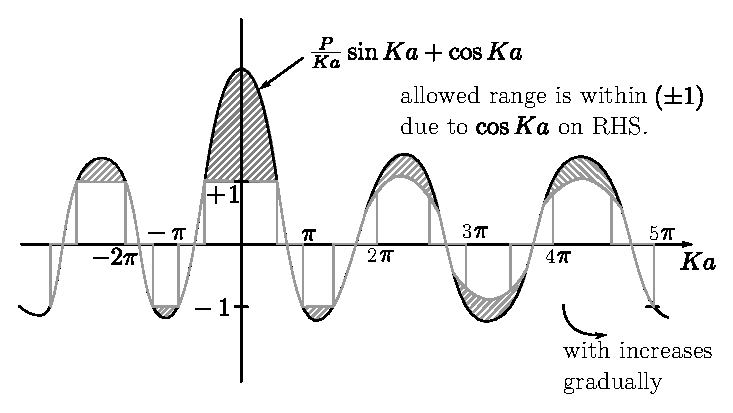
\includegraphics{chap6/fig3.eps}
\end{figure}\pageoriginale
as well as a commutative diagram
\begin{figure}[H]
\centering
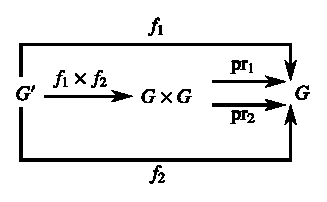
\includegraphics{chap6/fig4.eps}
\end{figure}
Therefore for any $a\in H^{1}_{\DR}(G/R)$, we have
$$
f^{*}_{3}(a)-f^{*}_{1}(a)-f^{*}_{2}(a)=(f_{1}\times f_{2})^{*}(\text{sum}^{*}(a)-\pr_{1}^{*}(a)-\pr_{2}^{*}(a)).
$$
In particular, if $a\in D(G/R)$, then $f^{*}_{3}(a)=f^{*}_{1}(a)+f^{*}_{2}(a)$.
\end{proof}

For the remainder of this section, we will consider a ring $R$ which is flat over $Z$, and an ideal $I\subset R$ which has divided powers. The flatness means that if we denote by $K$ the $Q$-algebra $R\otimes Q$, then $R\subset K$. That the ideal $I\subset R$ has divided powers means that for any integer $n\geq 1$, and any element $i\in I$, the element $i^{n}/n!$ of $K$ actually lies in $I$.

Given a formal Lie variety $V$ over $R$, we denote by $V\otimes K$ the formal Lie variety over $K$ obtained by extension of scalars. In terms of coordinates $X_{1},\ldots,X_{n}$ for $V$, $A(V\otimes K)$ is the power-series ring $K[[X_{1},\ldots,X_{n}]]$. We say that an element of $A(V\otimes K)$ is {\em integral} if it lies in the subring $A(V)$; similarly, an element of the de Rham complex $\Omega_{V\otimes K/K}$ is said to be {\em integral} if it lies in the subcomplex $\Omega_{V/R}$.

\medskip
\noindent
{\bf Lemma \thnum{5.1.2}.\label{art6-lem5.1.2}}~{\em Let $(V,0)$ be a pointed Lie variety over a $Z$-flat ring $R$. Then exterior differentiation induces an isomorphism of $R$-modules}
$$
\frac{\{f\in A(V\otimes K)|f(0)=0,df\text{ integral}\}}{\{f\in A(V)|f(0)=0\}}\xrightarrow{\sim}H^{1}_{\DR}(V/R)
$$
{\em which is compatible with morphisms of pointed Lie varieties.}

\begin{proof}
Because\pageoriginale $K$ is a $Q$-algebra, the formal Poincare lemma gives $H^{0}_{\DR}(V\otimes K/K)=K$, $H^{i}_{\DR}(V\otimes K/K)=0$ for $i\geq 1$. Therefore any closed one-form on $V/R$ can be written as df with $f\in A(V\otimes K)$, and this $f$ is unique up to a constant. If we normalize $f$ by the condition $f(0)=0$, we get the asserted isomorphism.
\end{proof}

\smallskip
\noindent
{\bf Key Lemma \thnum{5.1.3}.\label{art6-keylem5.1.3}}~{\em Let $(V,0)$ and $(V',0)$ be pointed formal Lie varieties over a $Z$-flat ring $R$, and let $I\subset R$ be an ideal with divided powers. If $f_{1}$, $f_{2}$ are two pointed morphisms $V'\to V$ such that $f_{1}=f_{2}$ mod $I$, then the induced maps}
$$
f^{*}_{1}, f^{*}_{2} : H^{1}_{\DR}(V/R)\to H^{1}_{\DR}(V'/R)
$$
{\em are equal.}
\smallskip

\begin{proof}
Let $\varphi_{1}$, $\varphi_{2}$ denote the algebra homomorphisms $A(V)\to A(V')$ corresponding to $f_{1}$ and $f_{2}$. By the previous lemma, we must show that for every element $f\in A(V\otimes K)$ with $f(0)=0$ and $df$ integral, the difference $\varphi_{1}(f)-\varphi_{2}(f)$ lies in $A(V')$, i.e. is itself integral. (Because $f_{1}$ and $f_{2}$ were assumed pointed, this difference automatically has constant term zero).

In terms of pointed coordinates $X_{1},\ldots,X_{n}$ for $V'$ and $Y_{1},\ldots,Y_{m}$ for $V$, the maps $\varphi_{1}$ and $\varphi_{2}$ are given by substitutions
\begin{align*}
\varphi_{1}(f(Y)) &=f(\varphi_{1}(X))\\
\varphi_{2}(f(Y)) &= f(\varphi_{2}(X))
\end{align*}
where $\varphi_{1}(X)$, $\varphi_{2}(X)$ are $m$-tuples of series in $X=(X_{1},\ldots,X_{n})$ without constant term. The hypothesis $f_{1}=f_{2}$ mod $I$ means that the component-by-component difference $\Delta=\varphi_{2}(X)-\varphi_{1}(X)$ satisfies 
$$
\Delta(0)=0, \Delta\text{~ has all coefficients in $I$}.
$$
We now compute using Taylor's formula, and usual multi-index notations:
\begin{align*}
\varphi_{2}(f) -\varphi_{1}(f) &= f(\varphi_{2}(X))-f(\varphi_{1}(X))\\
&= f(\varphi_{1}(X)+\Delta)-f(\varphi_{1}(X))\\
&=\sum\limits_{|\underline{n}|\geq 1}\frac{\Delta^{\underline{n}}}{(\underline{n})!}\left(\frac{\partial^{\underline{n}}}{\partial Y^{\underline{n}}}f\right)(\varphi_{1}(X)).
\end{align*}
This\pageoriginale last sum is $X$-adically convergent (because $\Delta$ has no constant term), and its individual terms are integral (because $\Delta$ has coefficients in the divided power ideal $I$, the terms $\Delta^{\underline{n}}/(\underline{n})!$ all have coefficients in $I$, and hence in $R$; because $df$ is integral, all the first partials $\partial f/\partial Y_{i}$ are integral, and a fortiori all the higher partials are integral).
\end{proof}

\medskip
\noindent
{\bf Theorem \thnum{5.1.4}.\label{art6-thm5.1.4}}~{\em Let $R$ be a $Z$-flat ring, and $I\subset R$ a divided power ideal. Let $G$, $G'$ be commutative formal Lie groups over $R$, and denote by $G_{0}$, $G'_{0}$ the commutative formal Lie groups over $R_{0}=R/I$ obtained by reduction mod $I$.}
\begin{itemize}
\item[(1)] {\em If $f:G'\to G$ is any morphism of pointed formal Lie varieties whose reduction mod $I$, $f_{0}:G'_{0}\to G_{0}$, is a group homomorphism, then the induced map $f^{*}:H^{1}_{\DR}(G/R)\to H^{1}_{\DR}(G'/R)$ maps $D(G/R)$ to $D(G'/R)$.}

\item[(2)] {\em If $f_{1}$, $f_{2}$, $f_{3}$ are three maps $G'\to G$ of pointed formal Lie varieties whose reductions mod $I$ are group homomorphisms which satisfy $(f_{3})_{0}=(f_{1})_{0}+(f_{2})_{0}$ in $\Hom(G'_{0},G_{0})$, then for any element $a\in D(G/R)$ we have}
$$
f^{*}_{1}(a)+f^{*}_{2}(a)=f^{*}_{3}(a).
$$
\end{itemize}

\begin{proof}
If $f:G'\to G$ is a pointed map which reduces mod $I$ to a group homomorphism, the diagram
\[
\xymatrix{
G'\times G'\ar[d]^-{f\times f}\ar[r]^-{\text{sum}} & G'\ar[d]^-{f}\\
G\times G\ar[r]^-{\text{sum}} & G
}
\]
commutes mod $I$, i.e.
$$
\text{sum~} (f\times f)\equiv f\text{~sum}\quad \mod I.
$$
and hence for any $a\in H^{1}_{\DR}(G/R)$ we have, by the previous lemma,
$$
(f\times f)^{*}(\text{sum}^{*}(a))=\text{sum}^{*}(f^{*}(a))
$$
The analogous diagrams with ``sum'' replaced by $\pr_{1}$ or $\pr_{2}$ commute, hence
$$
(f\times f)^{*}(\pr_{i}^{*}(a))=\pr^{*}_{i}(f^{*}(a))\quad\text{for~ } i=1,2.
$$\pageoriginale
Combining these, we find
\begin{align*}
& (f\times f)^{*}(\text{sum}^{*}(a)-\pr^{*}_{1}(a)-\pr^{*}_{2}(a))=\\
& \text{sum}^{*}(f^{*}(a))-\pr^{*}_{1}(f^{*}(a))-\pr^{*}_{2}(f^{*}(a)).
\end{align*}
In particular, if $a\in D(G/R)$ then $f^{*}(a)\in D(G'/R)$.

Similarly, if $f_{1}$, $f_{2}$ and $f_{3}$ are as in the assertion of the theorem, the diagram
\begin{figure}[H]
\centering
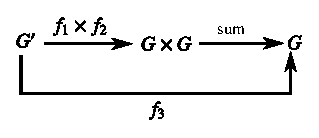
\includegraphics{chap6/fig5.eps}
\end{figure}
commutes mod $I$, and the diagram
\begin{figure}[H]
\centering
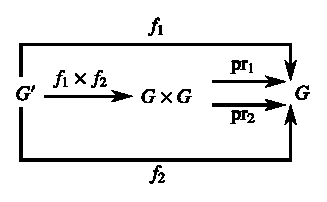
\includegraphics{chap6/fig4.eps}
\end{figure}
commutes. So again using the preceding lemma, we see that for any $a\in H^{1}_{\DR}(G/R)$, we have
$$
f^{*}_{3}(a)-f^{*}_{1}(a)-f^{*}_{2}(a)=(f_{1}\times f_{2})^{*}(\text{Sum}^{*}a)-\pr^{*}_{1}(a)-\pr^{*}_{2}(a)).
$$
In particular, for $a\in D(G/R)$, we obtain the asserted formula
$$
f^{*}_{3}(a)=f^{*}_{1}(a)+f^{*}_{2}(a).
$$
\end{proof}

Let $CFG(R;R_{0})$ denote the additive category whose {\em objects} are the commutative formal Lie groups over $R$, but in which the morphisms are the homomorphisms between their reductions mod $I$:
$$
\Hom_{CFG(R,R_{0})}(G',G)=\Hom(G'_{0},G_{0}).
$$
Given a homomorphism $f_{0}:G'_{0}\to G_{0}$, it always lifts to a pointed morphism\pageoriginale $f:G'\to G$ of formal Lie varieties (just lift its power-series coefficients one-by-one, and keep the constant terms zero).

According to the theorem, the induced map
$$
f^{*}:D(G/R)\to D(G'/R)
$$
is {\em independent} of the choice of pointed lifting $f$ of $f_{0}$. So it makes sense to denote the induced map
$$
(f_{0})^{*}:D(G/R)\to D(G'/R).
$$

\medskip
\noindent
{\bf Theorem \thnum{5.1.5}.\label{art6-thm5.1.5}}~{\em Let $R$ be a $Z$-flat ring, and $I\subset R$ a divided power ideal. Then the construction $G\mapsto D(G/R)$, $f_{0}\mapsto (f_{0})^{*}=$ (any pointed lifting)$^{*}$ defines a contravariant additive functor from the category $CFG(R;R_{0})$ to the category of $R$-modules.}
\smallskip

\begin{proof}
This is just a restatement of the previous theorem.
\end{proof}

\begin{remarks*}
\begin{itemize}
\item[(1)] Thanks to Lazard \cite{art6-key33}, we know that every commutative formal Lie group $G_{0}$ over $R_{0}$ lifts to a commutative formal Lie group $G$ over $R$. If $G'$ is another lifting of $G_{0}$, then the identity endomorphism of $G_{0}$ is an isomorphism of $G'$ with $G$ in the category $CFG(R;R_{0})$. Formation of the induced isomorphism $D(G/R)\xrightarrow{\sim}D(G'/R)$ provides a transitive system of identifications between the $D$'s of all possible liftings. In this way, it is possible to view the construction
$$
G_{0}\mapsto D(G/R),\text{~ where $G$ is some lifting of $G_{0}$}
$$
as providing a contravariant additive functor from $CFG(R_{0})$ to the category of $R$-modules. We will not pursue that point of view here.

\item[(2)] Even without appealing to Lazard, one can proceed in an elementary fashion by observing that any commutative formal Lie group $G_{0}$ over $R_{0}$ can certainly be lifted to a formal Lie ``monoid with unit'' $M$ over $R$ (simply lift the individual coefficients of the group law, and always lift $0$ to $0$). For a monoid, one can still define $D(M/R)$ as the primitive elements of $H^{1}_{\DR}(M/R)$, and one can still show exactly as before that the construction
$$
G_{0}\to D(M/R),\quad M\text{~ any monoid lifting of $G_{0}$}
$$
defines\pageoriginale a contravariant additive functor from $CFG(R_{0})$ to $R$-modules.
\end{itemize}
\end{remarks*}

\noindent
{\em A variant.} The reader cannot have failed to notice the purely formal nature of most of our arguments. We might as well have begun with {\em any} contravariant functor $H$ from formal Lie varieties over a $Z$-flat ring $R$ to $R$-modules for which the key lemma (\ref{art6-keylem5.1.3}) holds. One such $H$, which we will denote $H^{1}_{\DR}(V/R;I)$, is defined as $H^{1}$ of the {\em subcomplex} of the de Rham complex of $V/R$
$$
``IA(V)''\to \Omega^{1}_{V/R}\to \Omega^{2}_{V/R}\to \ldots
$$
where ``$IA(V)$'' denotes the kernel of reduction mod $I$:
$$
``IA(V)''=\Ker(A(V)\twoheadrightarrow A(V_{0})).
$$
In terms of coordinates for $V$, ``$IA(V)$'' is the ideal consisting of those series all of whose coefficients lie in $I$. The analogue of lemma (\ref{art6-lem5.1.2}) becomes
$$
\frac{\{f\in A(V\otimes K)|f(0)=0,dt\text{~integral}\}}{\{f\in ``IA(V)''|f(0)=0\}}\xrightarrow{\displaystyle{\mathop{\sim}\limits^{d}}}H^{1}_{\DR}(V/R;I).
$$
This much makes sense for {\em any} ideal $I\subset R$. If $I$ has divided powers, then the proof of the key lemma (\ref{art6-lem5.1.3}) is almost word-for-word the same. (It works because the terms $\Delta^{\underline{n}}/(\underline{n})!$ all have coefficients in $I$.)

The corresponding theory, ``primitive elements in $H^{1}_{\DR}(G/R;I)$,'' is denoted $D_{1}(G/R)$. In terms of coordinates $X=(X_{1},\ldots,X_{n})$ for $G$, we have the explicit description
\begin{multline*}
D_{1}(G/R)=\\
=\frac{\{f\in K[[X]]|f(0)=0,df\text{~integral, } f(X{\displaystyle{\mathop{+}\limits_{G}}Y})-f(X)-f(Y)\in I[[X,Y]]\}}{\{f\in I[[X]]|f(0)=0\}}
\end{multline*}
as compared with the explicit description
\begin{multline*}
D(G/R)=\\
=\frac{\{f\in K[[X]]|f(0)=0,df\text{~integral, } f(X{\displaystyle{\mathop{+}\limits_{G}}Y})-f(X)-f(Y)\text{~integral}\}}{\{f\in R[[X]]|f(0)=0\}}
\end{multline*}
For\pageoriginale ease of later reference we summarize the above discussion in a theorem.

\medskip
\noindent
{\bf Theorem \thnum{5.1.6}.\label{art6-thm5.1.6}}~{\em Let $R$ be a $Z$-flat ring, and $I\subset R$ a divided power ideal. The key lemma (\ref{art6-lem5.1.3}) holds for $H^{1}_{\DR}(V/R;I)$, and theorems \eqref{art6-thm5.1.4} and \eqref{art6-thm5.1.5} hold for $D_{1}(G/R)$.}
\smallskip

The natural map $D_{1}\to D$ is not an isomorphism, but its kernel and cokernel are visibly killed by $I$. In the work of Honda and Fontaine, it is $D_{1}$ rather than $D$ which occurs; in the work of Grothendieck and Mazur-Messing (\cite{art6-key17}, \cite{art6-key35}), it is $D$ which arises more naturally.

Let us denote by $\underline{\omega}_{G/R}$ the $R$-module of translation-invariant, or what is the same, primitive, one-forms on $G/R$. Because $G$ is commutative, every element $w\in \underline{\omega}_{G/R}$ is a closed form, so we have natural maps
\[
\xymatrix{
\underline{\omega}_{G/R}\ar[r] & D_{1}(G/R)\ar[d]\\
                              & D(G/R)
}
\]
(Notice that in the extreme case $I=(0)$, the map $\underline{\omega}\to D_{1}$ is an isomorphism!)

\medskip
\noindent
{\bf Lemma \thnum{5.1.7}.\label{art6-lem5.1.7}}~{\em Suppose $R$ flat over $Z$, and $I\subset R$ an ideal. We have exact sequences}
\begin{align*}
& 0\to \Hom_{R\text{-groups}}(G,G_{a})\xrightarrow{d}\underline{\omega}_{G/R}\to D(G/R)\\
& 0\to |Hom_{R/I\text{-groups}}(\foprod{G}{(R/I)}{R},(G_{a})_{R/I})\to D_{1}(G/R)\to D(G/R)
\end{align*}

\begin{proof}
The first is the special case $I=0$ of the second; the second is clear from the explicit description of $D_{1}$ and $D$ given above.
\end{proof}

\medskip
\noindent
{\bf Corollary \thnum{5.1.8}.\label{art6-coro5.1.8}}~{\em If $\Hom_{R\text{-groups}}(G,G_{a})=0$, then the natural maps}
$$
\underline{\omega}_{G}\to D_{1}(G/R)\quad\text{and}\quad \underline{\omega}_{G}\to D(G/R)
$$
{\em are injective.}
\smallskip

The reader interested in obtaining the limit formula for Jacobi sums conjectured\pageoriginale
%page 195


